\documentclass[12pt,a4paper,parskip]{scrartcl}
\usepackage[utf8]{inputenc}
\usepackage[T1]{fontenc}
\usepackage[ngerman]{babel}
\usepackage{lmodern}
\usepackage[babel,german=guillemets]{csquotes}
\usepackage[style=verbose-ibid,backend=bibtex8]{biblatex}
\bibliography{baclit280114}
\usepackage{amsmath}
\usepackage{amsfonts}
\usepackage{amssymb}
\usepackage{makeidx}
\usepackage{graphicx}
\usepackage{url}
\usepackage[locale=DE]{siunitx}%SI Einheiten etc.
\usepackage[german]{fancyref}%möglicherweise rausnehmen oder justieren
\usepackage{booktabs} %Tabellen Horizontale Linier dick darstellen
\usepackage{rotating}
\usepackage{lscape}
\usepackage{subfig}
\usepackage[left=3cm,right=3cm,top=2cm,bottom=2cm]{geometry}
\begin{document}
\subsection{Spannungsvektor und Spannungstensor}
Zum besseren Verständnis was für Kräfte und Spannungsverhältnisse bei Umformvorgängen im Material vorherrschen ist es sinnvoll sie an infinitesimal kleinen Volumenelementen zu modellieren. Dazu stellt man sich einen Körper unter Belastung der Einzelkräfte $ F_i $ und der Flächenlasten $ p $ \ vor ( siehe \fref{fig:normalvektor}) \footcite [Vgl.][43]{tmr}. Äußere Belastungen verursachen grundsätzlich auch innere Kräfte in einem Bauteil. Betrachtet man den Schnitt s--s \begin{figure}[!htb]
  \centering
  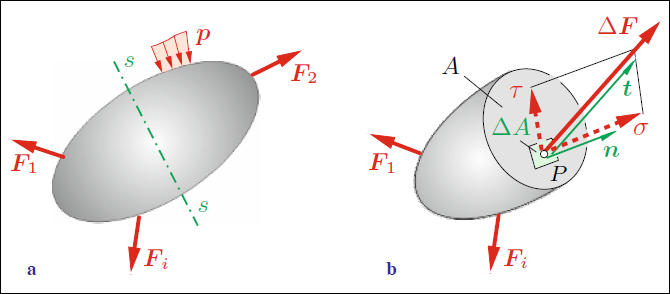
\includegraphics[scale=.8] {normalvektor}
  \caption{Spannungsvektor an beliebigen Körper}
  \label{fig:normalvektor}
  \end{figure} erkennt man das die inneren Kräfte sowie Spannungen über die ganze Schnittfläche $ A $ verteilt sind. Spannung sind über die Schnittfläche veränderlich deshalb  wird ein beliebiger Punkt $ P $ der Schnittfläche definiert. Die Schnittkraft $ \Delta F $  wirkt auf ein Flächenelement $ \Delta A $ (in dem $ P $ enthalten ist). Es wirkt eine gleich große entgegengesetzte Kraft auf die gegenüberliegende Schnittfläche (actio gleich reactio). Der Quotient $ \frac{\Delta F}{\Delta A} $ (Kraft auf die Fläche bezogen) definiert die mittlere Spannung für das Flächenelement. Wenn man nun bei der Beziehung $\frac{\Delta F}{\Delta A} $ den Differentialquotienten bildet in dem $ \Delt A \rightarrow 0 $ gegen Null läuft  resultiert daraus die Formel für den \emph{Spannungsvektor }$ t $ \begin{equation} t = \lim \limits_{\Delta A \to 0} \frac{\Delta F}{\Delta A} = \frac{\text{d}F}{\text{d}A} \end{equation}
Der Spannungsvektor lässt sich in eine Komponente normal zur Schnittfläche ( \emph{Normalspannung} $ \sigma $) und eine Komponente in der Schnittfläche (tangentiale \emph{Schubspannung} $ \tau $) zerlegen. Es existiert eine Abhängigkeit des Spannungsvektors $ t $ von der Lage des Punktes $ P $ in der Schnittfläche. Also eine Ortsabhängigkeit. Kann der Spannungsvektor $ t $ für alle Punkt von A angegeben werden, so ist die Spannungsverteilung in der Schnittfläche bekannt. Dennoch wird durch $ t $ der Spannungszustand in einem Punkt $ P $ nicht vollständig definiert. Werden durch $ P $ Schnitte in verschiedene Richtungen gelegt, so wirken entsprechend der unterschiedlichen Orientierung der Flächenelemente auch unterschiedliche Schnittkräfte. Es liegt demzufolge auch eine Schnittrichtungsabhängigkeit der Spannungen vor. Die Schnittrichtung wird von dem Normalenvektor $ n $ charakterisiert. Der Spannungszustand in einem Punkt $ P $ wird durch drei Spannungsvektoren in drei senkrecht aufeinander stehenden Schnittflächen festgelegt. Zu Darstellungszwecken fallen die drei Schnittflächen in dieser Modellierung mit den Koordinatenebenen eines kartesischen Koordinatensystems zusammen.

Um sie prägnant darzustellen, visualisiert man sie als Seitenflächen eines infinitesimalen Quaders mit den Kantenlängen d$ x $, d$ y $ und d$ z $ in der Umgebung von $ P $\begin{figure}[!htb]
  \centering
  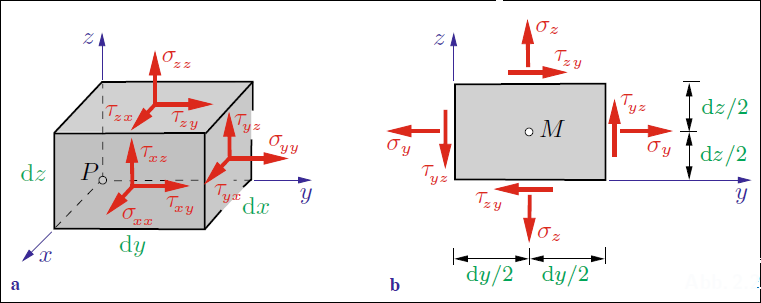
\includegraphics[scale=.7] {tensor}
  \caption{Spannungen und Kräfte am Infinitesimalelement}
  \label{fig:tensor}
  \end{figure}( siehe \fref{fig:tensor})\footcite[Vgl.][44]{tmr} . Ein Spannungsvektor wirkt hier je Fläche, der in seine Komponenten senkrecht zur Schnittfläche (daraus folgt Normalspannung) und in der Schnittfläche (daraus folgt Schubspannung) zerlegt wird. Zusätzlich werden die Schubspannungen noch in die Komponenten der Richtung der Koordinatenachsen zerlegt. Es werden Doppelindizes zur Kennzeichnung der jeweiligen Komponenten benutzt(siehe \fref{fig:tensor}). 
Der erste Index kennzeichnet die Richtung der Flächennormalen, wohingegen der zweite Index die Richtung der Spannungskomponenten bezeichnet. Zum Beispiel deklariert $ \tau_{yx} $ die Schubspannung einer Ebene, deren Normale in $y$ - Richtung weist. Die Spannung zeigt hier in die $ x $ - Richtung (siehe \fref{fig:tensor}). Es ist sinnvoll und vermeidet Verwechselungen bei den Normalspannungen die Schreibweise zu simplifizieren. Spannung und Flächennormale besitzen in diesem Fall die gleiche Richtung. Daraus ergibt sich eine Übereinstimmung der beiden Indizes und es ist hinreichend nur einen Index anzugeben. Es ist also völlig ausreichend  folgende Angaben zu machen: $ \sigma_{xx} = \sigma_{x} $, $ \sigma_{yy} = \sigma_y $, $ \sigma_{zz} = \sigma_z $.

Der Spannungsvektor für die Schnittfläche, deren Normale in $ y $ - Richtung zeigt wir mit den oben angeführten Konventionen zu folgender Formel:
\begin{equation}
t = \tau_{yx}e_x + \sigma_ye_y + \tau_{yz}e_z
\end{equation}

Analog zu den Schnittgrößen existiert für die Spannungen eine \emph{Vorzeichenkonvention}:

"`\emph{Positive} Spannungen zeigen an einem positiven (negativen) Schittufer in die positive (negative) Koordinatenrichtung."'\footcite[45]{tmr}

Infolgedessen beanspruchen positive (negative) Normalspannungen den infinitesimalen Quader auf Zug (Druck). Nach Zerlegung der Spannungsvektoren in ihre Komponenten erhält man drei Normalspannungen ($ \sigma_x$, $ \sigma_y $, $ \sigma_z $) und sechs Schubspannungen ( $ \tau_{xy}, \tau_{xz}, \tau_{yx}, \tau_{yz}, \tau_{zx}, \tau_{zy} $), die jedoch nicht alle unabhängig voneinander sind. Um das zu beweisen wird das Momentengleichgewicht um eine zur $x$- Achse parallele Achse durch den Mittelpunkt des Quaders (siehe \fref{fig:tensor})aufgestellt. Unter der Berücksichtigung das Gleichgewichtsaussagen nur für Kräfte gelten, werden die Spannungen mit den zugeordneten Flächenelementen multipliziert.
\begin{equation}
\overset{\curvearrowleft}{M}: 2\,\frac{\text{d}y}{2}\,(\tau_{yz}\,\text{d}x\,\text{d}z) - 2\,\frac{\text{d}z}{2}\,(\tau_{zy}\, \text{d}x\,\text{d}y)\,= 0 \Rightarrow\,\tau_{yz} = \tau_{zy}
\end{equation} Analog dazu gilt für die anderen Achsen: \begin{equation}
\tau_{xy}=\tau_{yx},\quad\tau_{xz}=\tau_{zx},\quad\tau_{yz}=\tau_{xy}
\end{equation}

Aus dem folgt:

"`Schubspannungen in zwei senkrecht aufeinander stehenden Schnitten (z.B. $\tau_{xy}$ und $\tau_{zy}$) sind gleich."'\footcite[46]{tmr}

Sie werden als einander \emph{zugeordnete Schubspannungen} bezeichnet. Aufgrund der Tatsache das sie gleiche Vorzeichen besitzen, deuten sie entweder auf die gemeinsame Quaderkante oder sie sind beide von ihr abgewandt. Wie aus den oben angeführten Identitäten zu erkennen ist, existieren lediglich sechs unabhängige Spannungen. Die Komponenten der jeweiligen Spannungsvektoren lassen sich in einer Matrix anordnen:
\begin{equation}
\sigma = \begin{pmatrix}
\sigma_x & \tau_{xy} & \tau_{xz}\\
\tau_{yx} & \sigma_y & \tau_{yz}\\
\tau_{zx} & \tau_{zy} & \sigma_z
\end{pmatrix} = \begin{pmatrix}
\sigma_x & \tau_{xy} & \tau_{xz}\\
\tau_{xy} & \sigma_y & \tau_{yz}\\
\tau_{xz} & \tau_{yz} & \sigma_z
\end{pmatrix}
\end{equation}

Die Normalspannungen bilden die Hauptdiagonale. Alle anderen Elemente sind Schubspannungen. Die Matrix ist symmetrisch und stellt den \emph{Spannungstensor} dar. Er wird mit der Größe $ \sigma $ bezeichnet. Der \emph{Spannungszustand} wird durch den \emph{Spannungstensor} (Spannungsvektoren für drei aufeinander stehende Schnitte) eindeutig in einem Punkt festgelegt.\footcite[Vgl.][43-46]{tmr}






\end{document}  